%        File: HW.tex
%     Created: 二 7月 03 12:00 下午 2018 C
% Last Change: 二 7月 03 12:00 下午 2018 C
%
\documentclass[UTF8,noindent]{ctexart}
\usepackage[a4paper,left=2.0cm,right=2.0cm,top=2.0cm,bottom=2.0cm]{geometry}
\usepackage{hyperref}
\usepackage{url}
\usepackage{graphicx}
\usepackage{amsmath}
\usepackage{amssymb}
\usepackage{enumitem}
\usepackage{tikz}
\usepackage{float}
\usepackage{listings}
\usepackage{xcolor}
\lstset{language = c,numbers=left, keywordstyle= \color{ blue!70 },commentstyle=\color{red!50!green!50!blue!50}, frame=shadowbox, rulesepcolor= \color{ red!20!green!20!blue!20 } 
} 
\usetikzlibrary{graphs}
\title{$Chapter\ 8-HW03$}
\author{$2015K8009929049$\ 冯吕}
\date{\today}
\begin{document}
\maketitle
\zihao{5}
\CJKfamily{zhsong}
$8.6.1$解:
\begin{itemize}
  \item $(1)\ x = a + b*c$:
	\begin{align*}
	  \text{三地址代码为}:&\\
	  &t_1 = b *c\\
	  &x = a + t_1\\
	  \text{生成的目标代码为}:&\\
	  &LD\ R_1, b\\
	  &LD\ R_2, c\\
	  &MUL\ R_1, R_1, R_2\\
	  &LD\ R_3, a\\
	  &ADD\ R_1, R_1, R_3\\
	  &ST\ x, R_1
	\end{align*}
  \item $(4)\ a[i] = b[c[i]]$:
	\begin{align*}
	  \text{三地址代码为}:&\\
	  &t_1 = i*4\\
	  &t_2 = c[t_1]\\
	  &t_3 = t_2 *4\\
	  &a[t_1] = b[t_3]\\
	  \text{生成的目标代码为}:&\\
	  &LD\ R_1, i\\
	  &MUL\ R_1, R_1, 4\\
	  &LD\ R_2, c(R_1)\\
	  &MUL\ R_2, R_2, 4\\
	  &LD\ R_3, b(R_2)\\
	  &ST\ a(R_1), R_3
	\end{align*}
  \item $(6)\ *p++ = *q++$:
	\begin{align*}
	  \text{三地址代码为}:&\\
	  &*p = *q\\
	  &p = p+4\\
	  &q = q+4\\
	\text{生成的目标代码为}:&\\
	&LD\ R_1, q\\
	&LD\ R_2, 0(R_1)\\
	&LD\ R_3m p\\
	&ST\ 0(R_3), R_2\\
	&ADD\ R_1, R_1, 4\\
	& ADD\ R_3, R_3, 4
	\end{align*}
\end{itemize}

$8.8.1$解:寄存器冲突图如下:

\begin{figure}[H]
  \centering
  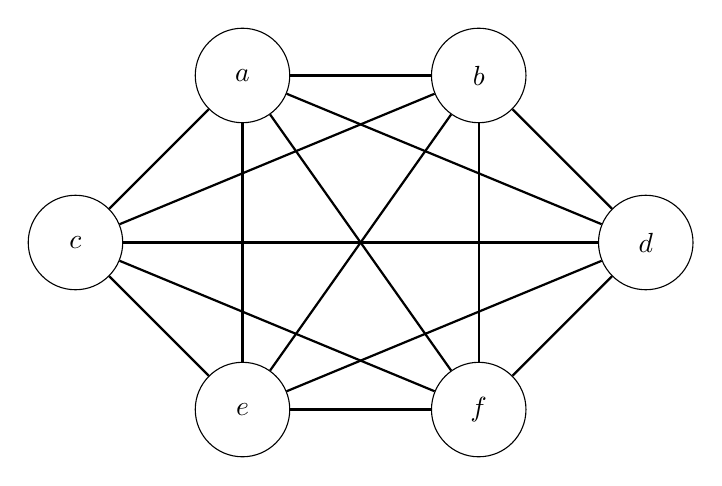
\begin{tikzpicture}[node distance = 3cm]
	\tikzstyle{nn} = [circle,draw = black, minimum size=12mm]
\tikzstyle{line} = [thick,>=stealth]
\node(a)[nn] {$a$};
\node(c)[nn,below left of = a ] {$c$};
\node(b)[nn, right of = a] {$b$};
\node(d)[nn, below right of = b] {$d$};
\node(e)[nn, below right of = c] {$e$};
\node(f)[nn, right of = e] {$f$};
\draw[line] (a) --(b);
\draw[line] (a) --(c);
\draw[line] (a) --(d);
\draw[line] (a) --(e);
\draw[line] (a) --(f);
\draw[line] (b) --(c);
\draw[line] (b) --(d);
\draw[line] (b) --(e);
\draw[line] (b) --(f);
\draw[line] (c) --(d);
\draw[line] (c) --(e);
\draw[line] (c) --(f);
\draw[line] (d) --(e);
\draw[line] (d) --(f);
\draw[line] (e) --(f);
  \end{tikzpicture}
\end{figure}

冲突图是一个包含$6$个节点的完全图。
\end{document}


